\documentclass{article}
\usepackage{amsmath}
\usepackage{mathtools}
\usepackage{txfonts}
\usepackage{fancyhdr}
\usepackage[margin=0.5in]{geometry}
\usepackage{graphicx}
\graphicspath{ {images/} }

\setlength{\parskip}{\baselineskip}%
\setlength{\parindent}{0pt}%
\pagestyle{fancy}
\fancyhf{}
\renewcommand{\headrulewidth}{0pt}

\begin{document}
\fancyhead[R]{\null\hfill\begin{tabular}[t]{l@{}}
	\textbf{Daniel Hartig} \\
	Stat 652 \\
	Homework 6
\end{tabular}}
\setlength{\headheight}{4\baselineskip}



\subsection*{Problem 1}
\subsubsection*{a.}
We use the N-P lemma to derive a MP test, where $x$ is the one observation of the test statistic $X$.
\begin{align*}
f(x|\theta_1) &= \mathcal{B}(1,1) = \frac{\Gamma(2)}{\Gamma(1)\Gamma(1)}x^0(1-x)^0 = 1 \\ \\
f(x|\theta_0) &= \mathcal{B}(2,2) = \frac{\Gamma(4)}{\Gamma(2)\Gamma(2)}x^0(1-x)^0 = 6x(1-x) \\ \\
\frac{f(x|\theta_1)}{f(x|\theta_0)} &= \frac{1}{6x(1-x)}
\end{align*}
A graph of this function over the range $(0,1)$ looks like:

\begin{center}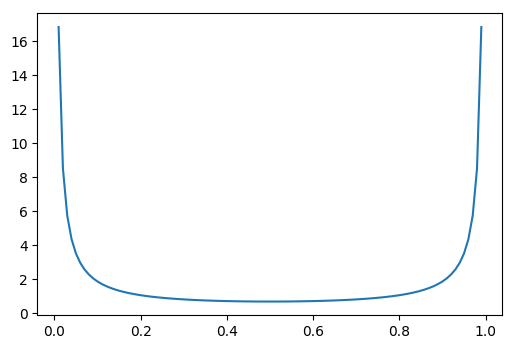
\includegraphics[scale=0.8]{hw6_1_graph}\end{center}

As we can see, the alternative hypothesis, being a uniform distribution, is much more likely than the null hypothesis at the edges of the distribution. The ratio increases for $X$ sufficiently close to the edge of the range $(0,1)$ ; therefore we should reject the null hypothesis for $X$ sufficiently close to the edges. Since $f(\mathbf{x}|\theta_0)$ is symmetric about $x=0.5$, we can solve for an $\alpha=0.05$ test on each side of the distribution. 
\begin{align*}
0.05 = \int^c_0 6x(1-x)dx &= 6\left.\left[\frac{x^2}{2}-\frac{x^3}{3}\right]\right|^c_0 \\
&=3c^2-2c^3 \\
-2c^3+3c^2-0.05 &= 0
\end{align*}
Using a numerical solver, the roots for this equation are ${-0.12407, 0.13535, 1.4882}$. Of these, the middle root is the only one that is sensible. Thus the rejection region for our test is $(0, 0.135)\cup(0.865, 1)$, and the test function is 
\[\phi(x) = \begin{cases} 1 & x\in (0, 0.135)\cup(0.865, 1) \\ 0 & \text{otherwise}
\end{cases}
\]
\subsubsection*{b.}
To calculate the p-value of an observation $x = 0.24$, we will integrate the null hypothesis distribution function from both edges to perform a 'two sided test.' Since this function is symmetrical as shown in section a, we can integrate one edge and double the answer. 
\begin{align*}
p &= 2\int_0^{0.24} 6x(1-x)dx \\
&=\left.\left[6x^2-4x^3\right]\right|^{0.24}_0 \\
&=0.290
\end{align*}

\subsection*{Problem 2}
\subsubsection*{a.}
For the null hypothesis that the balls are numbered 1-5, the mass function for $x$, the single observation of the test statistic $X$, is 
\[f(x|H_0) = \begin{cases} 0.2 & x = 1 \\ 0.2 & x = 2 \\ 0.2 & x=3 \\ 0.2 & x=4 \\ 0.2 & x=5 \\ 0 & \text{otherwise}\end{cases}\]
while fro the alternative hypothesis, the mass function for $x$ is
\[f(x|H_1) = \begin{cases} 1 & x = 5 \\ 0 & \text{otherwise}. \end{cases} \]
Using the N-P lemma to derive a MP test, we get a ratio of 
\[\frac{f(x|\theta_1)}{f(x|\theta_0)} = 5I_{\{5\}}(x).\]
From here we can build a table for our various cases

\begin{tabular}{ c c c }
$x$ & $f(x|\theta_1)/f(x|\theta_0)$ & $P_0(X=x)$ \\
1 & 0 & 0.2 \\
2 & 0 & 0.2 \\
3 & 0 & 0.2 \\
4 & 0 & 0.2 \\
5 & 5 & 0.2
\end{tabular}

The only sensisble rejection region is $x = 5$, but our size 0.1 test is not large enough to cover the entire $x = 5$ case. Therefore, there is a $0.1/0.2 = 0.5$ probabily of rejection when $x = 5$ amd the test function is 
\[\phi(x)=\begin{cases} 0.5 & x = 5 \\ 0 & \text{otherwise}\end{cases}\]
\subsubsection*{b.}
The power of the test is the probability of rejecting the null hypothesis when the alternative hypothesis is true. If the alternative hypothesis is true, then the only possible ball selection is $x=5$. From the test function in part a, we have a $0.5$ probability of rejecting the null hypothesis given that the alternative hypothesis is true. 

\subsection*{Problem 4}
To use the likelihood ratio test, we must calculate the supremum of likelihood ratios for each possible value of $\theta \in {2,4,6}$ for the null hypothesis. Therefore, we must calculate the distribution function for $f(x|\theta)$ for each value of $\theta$. These must be calculated with combinatorial rules for selecting balls from urns. The general formula for selecting $z$ different colored balls with $\theta$ colors and $y = 12/\theta$ balls of each color is
\begin{align*}
z = 1 \quad &\rightarrow \quad\binom{\theta}{1}\,\frac{\binom{y}{3}}{\binom{12}{3}} \\ 
z = 2 \quad &\rightarrow \quad2\,\binom{\theta}{2}\,\frac{\binom{y}{2}\binom{y}{1}}{\binom{12}{3}}
\end{align*}
For selecting all balls of one color, we must chose one color from $\theta$ available colors, and choose 3 balls from $y$ balls of that color. For selecting balls of two colors, we must choose two colors from $\theta$ availble, select 2 balls from the $y$ balls of one color, and 1 ball from the $y$ balls of the other color, then multiply by 2 to account for either color having 1 or two balls selected from it. The results of this are the following mass functions for each $\theta$. The mass functions assume that the probablility of any unlisted $x$ value is 0.
\begin{align*}
f(X|\theta=2) &= \begin{cases}0.1818 & x=1\\0.8182 & x=2 \end{cases} \\ 
f(X|\theta=3) &= \begin{cases}0.0545 & x=1 \\0.6545 & x=2 \\ 0.2909 & x=3 \end{cases} \\
f(X|\theta=4) &= \begin{cases}0.0182 & x=1 \\0.4909 & x=2 \\ 0.4909 & x=3 \end{cases} \\
f(X|\theta=6) &= \begin{cases}0.2727 & x=2 \\ 0.7273 & x=3 \end{cases} 
\end{align*}
Since we now have all values for any possible $x$ and $\theta$ combination, we can calculate 
\[\lambda(x) = \frac{\sup\limits_{\theta\in\{3\}}L(\theta|x)}{\sup\limits_{\theta\in\{2,4,6\}}L(\theta|x)}\]
for each possible $x$ in the table below

\begin{tabular}{ c c }
$x$ & $\lambda(x)$ \\
1 & $0.1818/0.0545 = 3.329$ \\
2 & $0.4909/0.6545 = 0.7450$\\
3 & $0.7273/0.2909 = 2.500$
\end{tabular}

We wish to reject if $\lambda(x)$ is sufficiently small, so we will reject when $x=2$. Under the null hypothesis, $P(x=2|\theta=3) = 0.6545$, so this is much larger than our size $0.1$ test. Therefore the probability of rejection when $x=2$ is $0.1/0.6545 = 0.1528$. The test function is
\[\phi(x)=\begin{cases}0.1528 & x=2 \\ 0 & \text{otherwise}\end{cases}\]

\subsection*{Problem 5}
By factorization we can find a sufficient statistic
\[f(\mathbf{x}|\theta) = \sum_{n=1}^2\frac{2x_i}{\theta^2}I_{(o,\theta]}(x_i) = \frac{4}{\theta^4}x_1x_2I_{(0, \theta^2]}(x_1x_2).\]
The sufficient statistic is $T(\mathbf{X}) = X_1X_2$. For all $\theta\in(0,\infty)$ where $\theta_1 > \theta_2$ we can use the likeihood ratios to show that 
\begin{align*}
\frac{f(t|\theta_2)}{f(t|\theta_1)} = \frac{\frac{4}{\theta_2^4}tI_{(0,\theta_2^2]}(t)}{\frac{4}{\theta_1^4}tI_{(0,\theta_1^2]}(t)} = \begin{cases}\infty & [\theta_1,\theta_2) \\ \left(\frac{\theta_1}{\theta_2}\right)^4 & (0, \theta_1^2). \end{cases}
\end{align*}
Since $\theta_1 > \theta_2$, we can see that the family of density functions of $T$ is monotone, non-decreasing. We then apply the Karlin-Rubin theorem to find a test that rejects $H_0$ if and only if $T < t_0$ which will be UMP level $\alpha$ for $\alpha = P_0(T>t_0)$. Under the null hypothesis, we set $\theta = 2.5$ and find 
\[P_{\theta = 2.5}(T<t_0) = F_T(t_0|\theta = 2.5) = \alpha\]
The distribution function of $T$ is calculated by 
\begin{align*}
F_T(t_0) &= \int_0^{t_0} f_T(t)dt = \frac{4}{\theta^4}\int_0^{t_0}tdt \\&= \frac{t_0^2}{\theta^4}
\end{align*}
This last expression is equal to $\alpha$. We are given $x_1 = 1.5; x_2 = 1.3$ so $t = x-1x_2 = 1.95$. Solving for alpha
\[\alpha = \frac{t_0^2}{\theta^4} = \frac{1.95^2}{2.5^4} = 0.0973\]
which is the $p$-value of this sample. This makes since because both $1.5$ and $1.3$ are well below the $\theta = 2.5$ upper limit of the distribution and this $p$-value makes it likely that we would reject the null hypothesis. If the $x_i$ values had been closer to, or exceeding, $2.5$, we would have expected a much higher $p$-value and to have accepted the null hypothesis. 

\subsection*{Problem 6}
By factorization, we can find a sufficient statistic for 
\begin{align*}
f(\mathbf{x}|\theta) &= \prod_{i=1}^n (\theta+1)x_i^\theta I_{(0,1)}(x) \\
&=(\theta+1)^n\left(\prod_{i=1}^n x_i\right)^\theta \prod_{i=1}^n I_{(0,1)}(x)
\end{align*} 
We can use $T(\mathbf{x}) = \prod_{i=1}^n x_i$ as a sufficent statistic. Since $1^n = 1$ and $0^n = 0$, the range of $t$ is the same as the range of $x$, so our joint distribution in terms of $t$ is 
\[f(t|\theta) = (\theta+1)^n(t)^\theta I_{(0,1)}(t) \]


\end{document}